\documentclass{article}

\usepackage[utf8]{inputenc}
\usepackage[english]{babel}
\usepackage{telecommunicatikz}

\begin{document}
  \begin{figure}
    \centering
    \begin{tikzpicture}
      \Device[Sample]{(2, 0)}{sample};
      \GeneratorSin{(0, 0)}{gen} % The semicolon can be omitted here.
      \amplifier[log]{(4, 0)}{logamp}

      \Line (gen) -- (sample) -- (logamp);
      \Line[-latex] (logamp.east) to +(1cm, 0) node[right] {To ADC};

      \MakeRegulated[$f$]{gen} % A generator with controlled frequency.
    \end{tikzpicture}
    \caption{\label{fig:Example} TelecommunicaTikZ usage example.}
  \end{figure}
\end{document}

